\documentclass[12pt,a4paper]{article}

\usepackage[T1]{fontenc}
\usepackage{amsmath, amssymb, amsfonts}
\usepackage[magyar]{babel}
\usepackage[utf8]{inputenc}
\usepackage{graphicx}
\usepackage{graphics}
\usepackage{mathtools}
\usepackage{epsfig}
\usepackage{epstopdf}
\usepackage{cite}
\usepackage{caption}
\usepackage{hyperref}
\usepackage[bottom=4cm]{geometry}
%\geometry{a4paper, portrait, margin=1in}

\renewcommand{\arraystretch}{1.3}

\title{\huge{Alkalmazott Fizikai Módszerek Laboratórium}\\ \vspace{20pt}
\textbf{Transzmissziós elektronmikroszkópia}}

\author{\Large{\textsc{Csörnyei Géza}} \vspace{10pt}\\
	\textrm{Eötvös Loránd Tudományegyetem}\\
	\textrm{Fizikus MSc I}
	}
\date{}
%\lhead{}
\begin{document}
\addtolength{\voffset}{-1.0cm}
\addtolength{\textheight}{1.0cm}
\begin{titlepage}
\maketitle

\begin{figure}[!htb]
\centering

\includegraphics[scale=0.6]{eltecimer.jpg}
\end{figure}

\hfil \Large{'E' mérőcsoport}\hfil  \\
\vspace*{2pt}
\hfil \Large{\emph{Mérés dátuma:} 2019.11.22.}\hfil \\
\vspace*{2pt}
\hfil \hspace*{45pt} \Large{\emph{Mérés vezetője:} Lábár János}\hfil
\thispagestyle{empty}
\end{titlepage}

\section{Rövid bevezető}
\hspace*{10pt} Mérésünk soorán a TEM (transzmissziós elektronmikroszkóp működési elvével ismerkedtünk meg, valamint lehetőségünk nyílt különböző minták diffrakciós mintázatának tanulmányozására is. Méréseink kalibrálása után indexeltem a hexagonális kristályrácsokról készített diffrakciós képeket, majd meghatároztam a zónatengelyeket, illetve a minták orientációját. Az indexeléshez a négyindexes hexagonális rendszert használtuk, melyre a szimmetria szerinti ekvivalenciákhoz való igazodás miatt volt szükség. Az indexelés hátterének, valamint számításának részletei megtalálhatók [1] jegyzetben, valamint [2] cikkben.

\section{Mérés menete}
\hspace*{10pt} A mérés során egy Al$_2$O$_3$ hordozóra növesztett GaN álló minta egymásra merőleges metszeteiről vettünk fel diffrakciós képeket. A felvett diffrakciós képeken is látszott, hogy mindkét minta hexagonális rendszerben kristályosodik. A mikroszkóp és a minta beállítását követően a Kikuchi-sávok mentén magas szimmetriájú pontokat keresve orientáltuk a mintát, majd mind a hordozó rétegről, mind a számunkra érdekes GaN rétegről diffrakciós képeket készítettünk, majd ezen lépéseket megismételtük a merőleges metszet esetén is.

\section{Mérések kiértékelése}
\hspace*{10pt} Méréseink kiértékeléséhez először kalibrálnunk kell a készült képeket. Ehhez a \texttt{Ni} mintáról készült polidiffrakciós képet értékeltük ki. A kalibrációt az alábbi egyenlet segítségével végezhetjük el, mivel ezen anyag köbös kristályráccsal rendelkezik:
\begin{equation}
R_{hkl} = \frac{L\lambda}{a}\sqrt{h^2+k^2+l^2},
\end{equation}
ahol $R_{hkl}$ a felvételen a direkt nyaláb és a $hkl$ indexű síksereg távolsága, $L$ a kalibrálandó kamerahossz, $\lambda$ a hullámhossz, $a$ pedig a rácsállandó. Mivel a rácstávolságok ezen szimmetriájú rács esetében 
\begin{equation}
d_{hkl} = \frac{a}{\sqrt{h^2+k^2+l^2}}
\end{equation}
alakban adhatjuk meg, így a két összefüggés összevetésével látható, hogy a diffrakciós képen mért távolságok fordítottan arányosak a valós rácssíktávolságokkal. A kalibrációs képen az egyes gyűrűk sugarát megmérve, majd ezen távolságokat összevetve a hozzájuk tartozó rácssíktávolságokkal meghatározhatjuk a rendszer mikroszkóp állandóját, mely segítségével elvégezhetjük a többi minta indexelését.
\hspace*{10pt} A kalibráció elvégzéséhez kinyomtattam az egyes diffrakciós képeket, majd egy vonalzó segítségével megmértem az egyes diffrakciós körök átmérőit, ahogy a függelék első ábráján is látszik. Az egyes mért értékekhez párosítani tudjuk az egyes rácssíktávolságokat a \texttt{Ni} kalibrációs lapjának segítségével. A mért távolságok valamint a hozzájuk tartozó rácssíktávolságok a \ref{tab:kalib}. táblázatban láthatók.\\
\begin{table}[!h]
\begin{center}
\begin{tabular}{|c|c|c|}
\hline
R [mm] & d [\AA] & 1/d [1/\AA]\\
\hline
27.5 & 2.03718 & 0.49087\\
\hline
32.0 & 1.76425 & 0.56681\\
\hline
45.0 & 1.24751 & 0.80160\\
\hline
53.0 & 1.06388 & 0.93996\\
\hline
71.0 & 0.80949 & 1.23534\\
\hline
\end{tabular}
\caption{A kalibrációhoz szükséges értékek táblázata. Az általam feljegyzett utolsó távolságot megelőzően még kettő további diffrakciós gyűrűnek is látszódnia kellett volna a kalibrációs lap szerint, melyek halványan látszódtak is a képen azonban a távolságok meghatározása bizonytalan lett volna, így  ezek elhagyása mellett döntöttem.}
\label{tab:kalib}
\end{center}
\end{table}
\newline
\hspace*{10pt} A táblázatban listázott pontokra a fenti
\begin{equation}
\frac{1}{d_{hkl}} = L\lambda \cdot R_{hkl}
\end{equation}
egyenlet értelmében egyenest illesztettem, majd ezen egyenes meredekségéből meghatároztam a mikroszkóp állandót, melyre $L\lambda$ = 0.0352 $\textrm{mm}\cdot$\AA \hspace{3pt} érték adódott. A továbbiakban ezen értéket leosztva a papíron mért értékekkel megkapjuk az egyes diffrakciós pontokhoz tartozó rácssíktávolságokat.\\
\begin{figure}[!h]
\centering
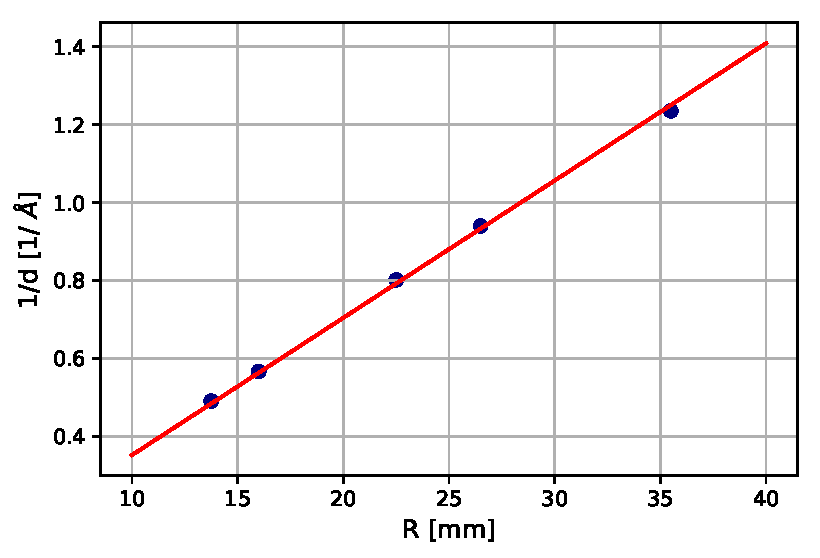
\includegraphics[width=0.7\linewidth]{kalib}
\caption{A mikroszkóp állandó meghatározásához készített kalibrációs egyenes}
\label{fig:kalib}
\end{figure}
\newpage
A rácssík távolságok ismeretében a mérés honlapján található JCPDS adatlapok segítségével meghatározhatjuk a diffrakciós pontok indexeit. A kapott (\emph{hkl}) indexekből az $i:=-(h+k)$ módon vezethetjük a hexagonális rendszereknél használatos négyes ($hkil$) indexelésre. A négyes indexelések esetében természetesen ugyanúgy teljesülnie kell a vektoriális összeadások szabályainak mint a háromindexes esetben.\\
Az egyes diffrakciós képek indexelését a 2-7. táblázatok tartalmazzák.
\begin{table}[!h]
\begin{center}
\begin{tabular}{|c|c|c|c|c|c|}
\hline
Pont indexe (\#) & R$_{\textrm{mért}}$ (mm) & d$_{\textrm{mért}}$ (\AA) & d$_{\textrm{valós}}$ (\AA) & $hkl$ & $hkil$ \\
\hline
1 & 12.0 & 2.367 & 2.379 & 110 & $11\overline{2}0$ \\
\hline
2 & 17.5 & 1.623 & 1.601 & $\overline{1}\overline{1}6$ & $ \overline{1}\overline{1}26 $\\
\hline
4 & 13.0 & 2.185 & 2.165 & 006 & 0006\\
\hline
\end{tabular}
\caption{Az Al$_2$O$_3$ hordozóról készített első diffrakciós kép kiértékelése (\texttt{Al2O3\_1.jpg})}
\end{center}
\end{table}


\begin{table}[!h]
\begin{center}
\begin{tabular}{|c|c|c|c|c|c|}
\hline
Pont indexe (\#) & R$_{\textrm{mért}}$ (mm) & d$_{\textrm{mért}}$ (\AA) & d$_{\textrm{valós}}$ (\AA) & $hkl$ & $hkil$ \\
\hline
1 & 10.0 & 2.840 & 2.760 & 100 & $10\overline{1}0$ \\
\hline
3 & 11.0 & 2.581 & 2.590 & 002 & 0002 \\
\hline
4 & 15.0 & 1.893 & 1.884 & 102 &$ 10\overline{1}2$\\
\hline
\end{tabular}
\caption{A $GaN$ hordozóról készített első diffrakciós kép kiértékelése (\texttt{GaN\_1.jpg})}
\end{center}
\end{table}


\begin{table}[!h]
\begin{center}
\begin{tabular}{|c|c|c|c|c|c|}
\hline
Pont indexe (\#) & R$_{\textrm{mért}}$ (mm) & d$_{\textrm{mért}}$ (\AA) & d$_{\textrm{valós}}$ (\AA) & $hkl$ & $hkil$ \\
\hline
1 & 8.0 & 3.545 & 3.479 & 012 & $01\overline{1}2$ \\
\hline
2 & 11.0 & 2.581 & 2.552 & $01\overline{4}$ &$ 01\overline{1}\overline{4}$ \\
\hline
3 & 13.0 & 2.184 & 2.165 & $00\overline{6}$ & $000\overline{6}$\\
\hline
\end{tabular}
\caption{Az Al$_2$O$_3$ hordozóról készített második diffrakciós kép kiértékelése (\texttt{Al2O3\_2.jpg})}
\end{center}
\end{table}

\newpage
\begin{table}[!h]
\begin{center}
\begin{tabular}{|c|c|c|c|c|c|}
\hline
Pont indexe (\#) & R$_{\textrm{mért}}$ (mm) & d$_{\textrm{mért}}$ (\AA) & d$_{\textrm{valós}}$ (\AA) & $hkl$ & $hkil$ \\
\hline
1 & 17.5 & 1.626 & 1.591 & 110 & $11\overline{2}0$ \\
\hline
2 & 21.0 & 1.352 & 1.357 & 112 & $11\overline{2}2$ \\
\hline
3 & 11.0 & 2.581 & 2.590 & 002 & 0002\\
\hline
\end{tabular}
\caption{A $GaN$ hordozóról készített második diffrakciós kép kiértékelése (\texttt{GaN\_2.jpg})}
\end{center}
\end{table}


\begin{table}[!h]
\begin{center}
\begin{tabular}{|c|c|c|c|c|c|}
\hline
Pont indexe (\#) & R$_{\textrm{mért}}$ (mm) & d$_{\textrm{mért}}$ (\AA) & d$_{\textrm{valós}}$ (\AA) & $hkl$ & $hkil$ \\
\hline
1 & 15.0 & 1.893 & 1.884 & 102 & $10\overline{1}\overline{2}$ \\
\hline
2 & 10.0 & 2.840 & 2.760 & 100 & $10\overline{1}0$ \\
\hline
3 & 11.0 & 2.581 & 2.590 & $00\overline{2}$ & $000\overline{2}$\\
\hline
\hline
$\widetilde{1}$ & 17.5 & 1.623 & 1.601 & 116 & $11\overline{2}6$\\
\hline
$\widetilde{2}$ & 12.0 & 2.366 & 2.379 & 110 & $11\overline{2}0$\\
\hline
$\widetilde{3}$ & 13.0 & 2.184 & 2.165 & $00\overline{6}$ & $000\overline{6}$\\
\hline
\end{tabular}
\caption{A $GaN$ (\#) és az Al$_2$O$_3$ ($\widetilde{\#}$) rétegekről készített első együttes diffrakciós kép kiértékelése (\texttt{Al2O3\_GaN\_1.jpg})}
\end{center}
\end{table}


\begin{table}[!h]
\begin{center}
\begin{tabular}{|c|c|c|c|c|c|}
\hline
Pont indexe (\#) & R$_{\textrm{mért}}$ (mm) & d$_{\textrm{mért}}$ (\AA) & d$_{\textrm{valós}}$ (\AA) & $hkl$ & $hkil$ \\
\hline
1 & 11.0 & 2.581 & 2.590 & 002 & 0002 \\
\hline
3 & 17.5 & 1.623 & 1.591 & $\overline{1}\overline{1}0$ & $\overline{1}\overline{1}20$ \\
\hline
4 & 21.0 & 1.352 & 1.357 & 112 & $11\overline{2}2$\\
\hline
\hline
$\widetilde{1}$ & 13.0 & 2.184 & 2.165 & 006 & 0006\\
\hline
$\widetilde{3}$ & 21.0 & 1.385 & 1.374 & $\overline{3}00$ & $\overline{3}030$\\
\hline
$\widetilde{4}$ & 24.5 & 1.159 & 1.160 & 306 & 30$\overline{3}6$\\
\hline
\end{tabular}
\caption{A $GaN$ (\#) és az Al$_2$O$_3$ ($\widetilde{\#}$) rétegekről készített második együttes diffrakciós kép kiértékelése (\texttt{Al2O3\_GaN\_2.jpg})}
\end{center}
\end{table}
\newpage
\hspace*{10pt} Hármas ($uvw$) indexek esetében a zónatengelyek irányát úgy kaphatjuk, hogy a diffrakciós síkban fekvő két vektor vektoriális szorzatát képezzük, majd ezt lenormáljuk a számhármas legnagyobb közös osztójával. Ez megfelel a Weiss-törvénynek, miszerint a zónatengely indexire teljesülnie kell a sík tetszőleges Miller-index-hármasával az alábbi relációnak:
\begin{equation}
uh+vk+wl=0
\end{equation}
Négyesindexű reciprokrács-vektorokból nem számíthatjuk a zónatengelyt vektoriális szorzattal, viszont ekkor a zónatengely irányát megkaphatjuk a háromindexes zónatengely segítségével a következő módon:
\begin{equation}
\begin{split}
u = \frac{1}{3}(2u' - v'),\\
v = \frac{1}{3}(2v' - u'),\\
t = -\frac{1}{3}(v' + u'),\\
w = w'
\end{split}
\end{equation}
A háromindexes zónatengelyeket a fent említett módon lehet számolni egy vektoriális szorzat segítségével. A háromindexes ($uvw$) jelölésből ezt követően a fent egyenletrendszer alapján lehet áttérni a négyindexes ($uvwt$) zónatengelyirányra (itt természetesen a négyindexes jelölés első két indexe nem egyezik meg a háromindexes jelölés első két indexével). A számolt zónatengelyeket a \ref{tab:zonat}. táblázat tartalmazza.\\

\begin{table}[!h]
\begin{center}
\begin{tabular}{|c|c|c|c|c|}
\hline
Diffrakciós kép & $h_1k_1l_1$ & $h_2k_2l_2$ & $uvw$ & $uvtw$ \\
\hline
Al$_2$O$_3$ 1. & 110 & $\overline{1}\overline{1}6$ & $1\overline{1}0$ & $1\overline{1}00$\\
\hline
GaN 1. & 100 & 002 & $0\overline{1}0$ & $1\overline{2}10$ \\
\hline
Al$_2$O$_3$ 2. & 012 & $01\overline{4}$ & $\overline{1}00$ & $\overline{2}110$ \\
\hline
GaN 2. & 110 & 112 & $1\overline{1}0$ & $1\overline{1}00$ \\
\hline
\hline
Al$_2$O$_3$+GaN 1. (GaN) & 102 & 100 & 010 & $\overline{1}2\overline{1}0$ \\
\hline
Al$_2$O$_3$+GaN 1. (Al$_2$O$_3$) & 116 & 110 & $\overline{1}10$ & $\overline{1}100$\\
\hline
\hline
Al$_2$O$_3$+GaN 2. (GaN) & 002 & $\overline{1}\overline{1}0$ & $\overline{1}10 $ & $\overline{1}100$ \\
\hline
Al$_2$O$_3$+GaN 2. (Al$_2$O$_3$) & 006 & $\overline{3}00$ & $0\overline{1}0$ & $1\overline{2}10$\\
\hline
\end{tabular}
\caption{A zónatengelyek irányait tartalmazó táblázat a különböző diffrakciós képek esetére}
\label{tab:zonat}
\end{center}
\end{table}
%\newline
\newpage
\hspace*{10pt} Az egyes diffrakciós indexeléseket összevetve azt kapjuk, hogy az egyetlen közös síksereg az Al$_2$O$_3$ hordozó esetében a 0006 síksereg, valamint a GaN réteg esetében a 0002 síksereg. Ez annak felel meg, hogy a hordozóban és a rétegben a reciproktér $z$-tengelye megegyezik. Ezt követően kiválasztottam az első metszet irányából készült felvételeket, majd tekintettem azon közös irányokat, melyek a fenti irányra merőlegesek. A közös irányokba álló síkok indexeinek típusa eltérő, Al$_2$O$_3$ hordozó esetén $11\overline{2}0$, míg a GaN réteg esetén $10\overline{1}0$. Ezen két síksereg közötti szög számolásával meghatározhatjuk azok orientációját. A számoláshoz azonban egy bonyolultabb képletre lesz szükségünk, mivel a síkseregek közötti szög nem azonos az irányok közötti szöggel. A számításokhoz a [2] cikkben felírt A2.6 képlettel számoltam:
\begin{equation}
\cos \Phi = \frac{hd+ke+\frac{1}{2}(he+kd)+\frac{3}{4}lg(a/c)^2}{(h^2+k^2+hk+\frac{3}{4}l^2(a/c)^2)^{1/2}}\cdot(d^2+e^2+de+\frac{3}{4}g^2(a/c)^2)^{1/2},
\end{equation}
ahol ($hkil$) az egyik síkhoz tartozó indexek, míg ($defg$) a másik síkhoz tartozó indexek, valamint $a$ és $c$ a hordozó és a réteg rácsparaméterei (a JCPDS adatlapok szerint ezek rendre 4.758 \AA\hspace*{3pt} és 3.186 \AA). A fenti képlet használatával $\cos \Phi = 0.866$ adódott, ezáltal a síkok által bezárt szög $\Phi \approx 30  ^{\circ}$-nak adódott.

\section{Diszkusszió}
\hspace*{10pt} A laborgyakorlat során megismerkedtünk a transzmissziós elektronmikroszkópia működési elveinek alapjaival, majd az általunk készített diffrakciós képekhez történő kalibrációt elvégezve meg tudtam határozni az egyes minták zónatengelyeinek irányát, valamint a mintában levő anyagok egymáshoz viszonyított orientációját is.

\section*{Hivatkozások}
\begin{itemize}
\item[(1).:] {http://metal.elte.hu/oktatas/alkfizlab/meresleirasok/TEM.pdf}
\item[(2).:] {https://www.energia.mta.hu/~labar/Edington.pdf}
\end{itemize}
\end{document}
